
%
%
%
%
%

\definecolor{color1}{RGB}{116, 184, 22}
\definecolor{color2}{RGB}{77, 171, 247}
\definecolor{color3}{RGB}{99, 230, 190}
\definecolor{color4}{RGB}{132, 94, 247}
\definecolor{color5}{RGB}{250, 176, 5}
	
	\begin{figure}[t] %
     \vspace{-4mm}
		\centering %
		\resizebox{0.9 \columnwidth}{!}{  %
			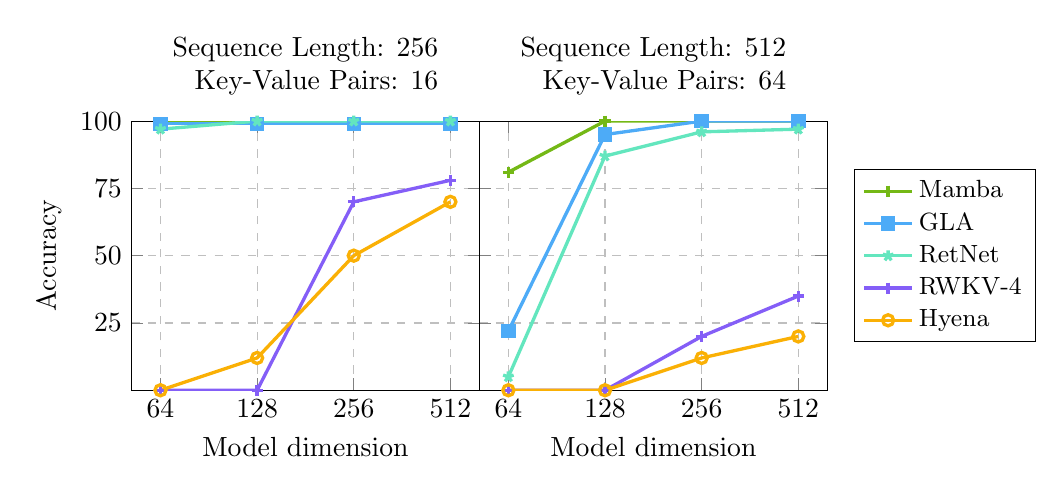
\begin{tikzpicture} %
			\scalefont{1.2} %
			\begin{axis}[
                name=plot1,
			sharp plot, %
        title style={align=right}, title={Sequence Length: 256\\Key-Value Pairs: 16},
    %
			xmode=normal,%
%
			xlabel=Model dimension, %
			ylabel=Accuracy, %
			width=6cm, height=5cm,  %
			%
			ymin=0, ymax=100,  %
			%
                symbolic x coords={64,128,256,512},
			ytick={25,50,75,100}, %
			xlabel near ticks, %
			ylabel near ticks, %
			ymajorgrids=true, %
                xmajorgrids=true,
			grid style=dashed, %
			]
			%
			\addplot+[very thick,mark=x,mark options={scale=0.5}, color=color1] plot coordinates { 
				(64,100)
				(128,100)
				(256,100)
				(512,100)
			};
			
			%
			\addplot+[very thick, mark=square*, mark options={scale=1}, color=color2] plot coordinates {
				(64,99)
				(128,99)
				(256,99)
				(512,99)
			};
			
			%
			\addplot+[very thick,mark=star,mark options={scale=1}, color=color3] plot coordinates {
				(64,97)
				(128,100)
				(256,100)
				(512,100)
			};
   			\addplot+[very thick,mark=+,mark options={scale=1}, color=color4] plot coordinates {
				(64,0)
				(128,0)
				(256,70)
				(512,78)
			};

			\addplot+[very thick,mark=o,mark options={scale=1}, color=color5] plot coordinates {
				(64,0)
				(128,12)
				(256,50)
				(512,70)
			};

			\end{axis}
			\begin{axis}[
                name=plot2,
                at={(plot1.south east) },
			sharp plot, %
        title style={align=right}, title={Sequence Length: 512\\Key-Value Pairs: 64},
			xmode=normal,%
%
			xlabel=Model dimension, %
			%
			width=6cm, height=5cm,  %
			%
			ymin=0, ymax=100,  %
                symbolic x coords={64,128,256,512},
   			ytick={0,25,50,75,100}, %
         yticklabels={,,},
			%
			xlabel near ticks, %
			%
			ymajorgrids=true, %
			xmajorgrids=true, %
			grid style=dashed, %
			legend style={at={(1.6,0.5)},anchor=east, legend cell align=left, font=\small}, 
			]
			
			\addplot+[very thick,mark=+,mark options={scale=1}, color=color1] plot coordinates { 
				(64,81)
				(128,100)
				(256,100)
				(512,100)
			};
			\addlegendentry{Mamba} 
			
			\addplot+[very thick, mark=square*, mark options={scale=1}, color=color2] plot coordinates {
				(64,22)
				(128,95)
				(256,100)
				(512,100)
			};
			\addlegendentry{GLA} 
			

			\addplot+[very thick, mark=star, mark options={scale=1}, color=color3] plot coordinates {
				(64,5)
				(128,87)
				(256,96)
				(512,97)
			};
			\addlegendentry{RetNet}  

			\addplot+[very thick, mark=+, mark options={scale=1}, color=color4] plot coordinates {
				(64,0)
				(128,0)
				(256,20)
				(512,35)
			};
			\addlegendentry{RWKV-4}  

		\addplot+[very thick, mark=o, mark options={scale=1}, color=color5] plot coordinates {
				(64,0)
				(128,0)
				(256,12)
				(512,20)
			};
			\addlegendentry{Hyena} 


			\end{axis}

			\end{tikzpicture}
		}
     \vspace{-3mm}
		%
		\caption{Accuracy (\%) on the synthetic MQAR task.} 
		\label{fig:mqar} 

	\end{figure}

